\chapter{Evaluatie/Discussie} \label{evaluatie}
In deze sectie wordt de ontwikkelde library ge\"evalueerd. Allereerst wordt er gekeken naar wat de impact van de library op de performance van de applicatie is \ref{performance}. Verder in dit hoofdstuk wordt de schaalbaarheid van de library bekeken \ref{schaalbaarheid}. Tot slot wordt er nog gekeken hoeveel effort er van de developer nodig is om de library te integreren in een applicatie \ref{Section:Effort}. Uit deze evaluaties wordt een conclusie getrokken over de Tracklytics library \ref{Section:Conclusie}.


\section{Performance Evaluatie} \label{performance}
In Hoofdstuk \ref{doelstelling} werd aangehaald dat impact van de Tracklytics library op de performance aanvaardbaar moet zijn om de applicatie niet significant te doen vertragen. In deze sectie wordt deze impact onderzocht en ge\"evalueerd. \\

Performance werd gemeten in twee verschillende applicaties, namelijk een stopwatch applicatie en een angry birds kloon \cite{AngryBirds}. De stopwatch wordt gebruikt omdat dit een niet-CPU-intensieve applicatie is en zo de resultaten niet vertekend zijn. De angry birds applicatie is CPU-intensiever en vereist een bepaalde framerate, aangezien dit een spel is. Deze applicatie wordt gebruikt  om de impact van de Tracklytics library op de framerate te onderzoeken. \\

Om te kijken welke extra vertraging de library heeft op de applicatie wordt de stopwatch applicatie gebruikt. Er wordt gekeken hoe lang het gemiddeld duurt om een functie oproep van een Tracklytics methode uit te voeren.\\

De angry birds applicatie wordt gebruikt om de impact van de library op de framerate van een spel te analyseren. Er wordt gekeken naar wanneer de framerate een significante daling ondervindt van het uitvoeren van simultane metingen. In deze analyse wordt er ook gekeken wat de invloed van het verlagen van het synchronisatie interval op de framerate betreft.\\

De evaluaties zijn uitgevoerd op een iPhone 6 \cite{iPhone} met als besturingssysteem: iOS versie 9.3.1. Het toestel was ten allen tijde voorzien van een WiFi verbinding met het internet. Om de resultaten op te halen van het toestel werd de ontwikkelaarsomgeving Xcode \cite{Xcode} versie 7.3.1 gebruikt.\\

In de volgende secties worden de metingen uitgelegd en uitgevoerd. Er gaat gemeten worden hoe lang de gemiddelde uitvoeringstijd bedraagt per methode die gebruikt kan worden van de library. Nadien wordt er gekeken naar de impact van de library op de framerate van de angry birds kloon.\\

\subsection{Call duration}
In deze sectie wordt uitgezocht hoelang het gemiddeld duurt voor elke methode van de Tracklytics library om volledig uitgevoerd te worden. Zo kan er ondervonden worden hoe groot de extra vertraging is die de library invoert in de applicatie. Deze test opstelling kan gezien worden als een benchmark. Om te testen hoe lang een methode gemiddeld duurt om uitgevoerd te worden, werd de volgende testopstelling uitgedacht. De geteste methode wordt X aantal keer uitgevoerd om hieruit een gemiddelde tijd te kunnen berekenen. Deze X wordt stelselmatig verhoogd om te kijken of de grootte van deze X een invloed heeft op de gemiddelde vertraging van de geteste methode. Deze testopstelling wordt gebruikt om alle beschikbare methodes in de Tracklytics library te evalueren. Het synchronisatieinterval is 60 seconden. \\

In de vorige secties werd beschreven dat de developer de keuze heeft tussen het tijdelijk opslaan van de metingen op de harde schijf van het toestel en het niet opslaan van de metingen op de harde schijf van het toestel. Dit heeft een invloed op de prestaties van de library, omdat er een significant prestatieverschil zit in disk I/O en verwerkingskracht \cite{diskIO}. Om dit prestatieverschil in kaart te brengen werd deze evaluatie uitgevoerd, eenmaal met het opslaan op disk en eenmaal zonder het opslaan op disk (aangegeven in de resultaten als ZOD).\\

Er werd in de Tracklytics library gekozen om de developer de vrijheid te geven om te beslissen dat de aggregatie van de metingen deels op het toestel van de gebruiker uitgevoerd wordt of dat deze aggregatie volledig uitgevoerd wordt in de back end. Omdat er een verschil bestaat in de implementatie van de geaggregeerde meetobjecten en de standaard meetobjecten zijn de testen opgedeeld in testen voor de standaard meetobjecten en testen voor de geaggregeerde meetobjecten (in het geval van de Gauge, de Meter en de Timer). Zo kunnen er de juiste conclusies getrokken worden uit de testen die uitgevoerd zijn.\\

\subsubsection{Bespreking resultaten}
In Hoofdstuk \ref{doelstelling} werd er besproken dat de impact van de ontwikkelde Tracklytics library op de performance van de applicatie zo minimaal mogelijk moet zijn. Indien we de onderstaande grafieken met de ruwe data uit de apendix \ref{Appendix} van de verschillende meetobjecten combineren zien we dat er zich bij het aanmaken van een niet-geaggregeerd meetobject telkens dezelfde trend voordoet: eerst daalt de tijd die nodig is om een meetobject aan te maken en deze tijd stijgt nadien weer naarmate er meer simultane metingen gebeuren. Aan de hand van de resultaten uit onderstaande grafieken en de tabellen kan geconcludeerd worden dat de library de grootste impact heeft op de applicatie indien de library de metingen op de harde schijf opslaat. Indien we gaan kijken naar de Counter tabel \ref{Table:Counter} zien we dat het aanmaken van een Counter gemiddeld \underline{+} 2000 keer sneller is indien het object niet op de harde schijf opgeslagen wordt. Dit resultaat geldt voor het aanmaken van elk niet-geaggregeerd meetobject. De \texttt{addEntry} methode bij de Meter maakt een Meter object aan en hoort dus bij het aanmaken van een niet-geaggregeerd meetobject. Indien we gaan kijken naar het snelheidsverschil bij het uitvoeren van een operatie op een niet-geaggregeerd meetobject, kunnen we vaststellen dat het verhogen en verlagen van een Counter \underline{+} 1000 maal sneller is indien de data niet op harde schijf wordt opgeslagen. Het stoppen van een Timer is \underline{+} 500 maal sneller indien deze Timer niet op de harde schijf van het toestel opgeslagen wordt. Uit deze observatie kunnen we concluderen dat de performance impact van de Tracklytics library groter is indien de metingen tijdelijk op de harde schijf opgeslagen worden. \\

Door naar de grafieken te kijken van de niet-geaggregeerde meetobjecten kunnen we zien dat er zich telkens dezelfde trend voordoet: de gemiddelde tijd die het inneemt om een meetobject aan te maken neemt toe naarmate er meer objecten aangemaakt worden en de hoeveelheid uitvoeringen van een methode op een meetobject heeft een beperkte invloed op de gemiddelde uitvoeringstijd van de methode. Deze observatie geldt zowel voor de metingen die opgeslagen worden op harde schijf als de metingen die niet opgeslagen worden op de harde schijf. Combineren we de grafieken met de resultaten in de tabellen kunnen we concluderen dat het aanmaken van Counters de zwaarste performance impact heeft. \\

\begin{figure}[h]
  \centering
  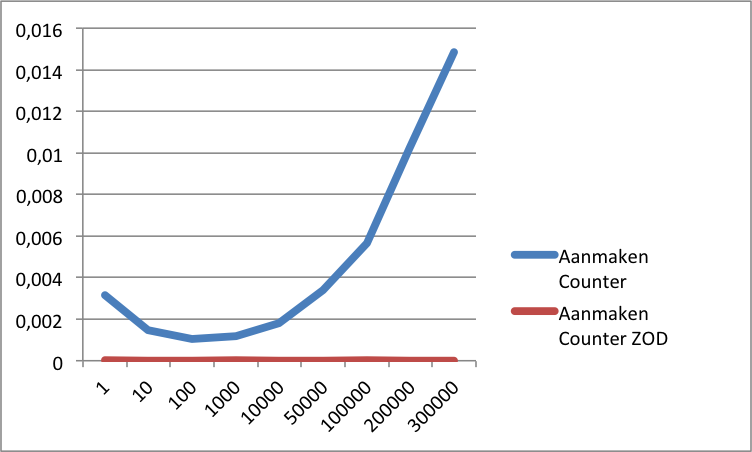
\includegraphics[scale=1.0]{Afbeeldingen/Evaluatie/AanmakenCounter}
  \caption{Grafiek vergelijking tijden aanmaken van een \texttt{Counter}.}
  \label{fig:GraphCounter}
\end{figure}

De figuur \ref{fig:GraphCounter} geeft de grafiek weer van het aanmaken van een \texttt{Counter} met en zonder het tijdelijk opslaan van deze \texttt{Counter} op de harde schijf.\\



\begin{figure}[h]
  \centering
  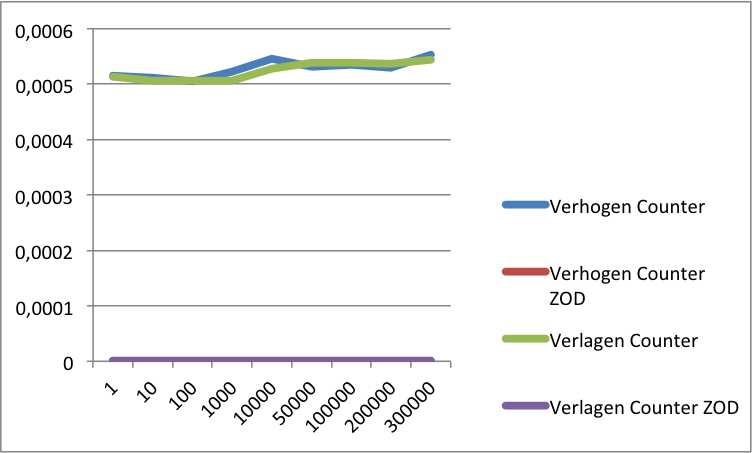
\includegraphics[scale=1.0]{Afbeeldingen/Evaluatie/VerhogenCounter}
  \caption{Grafiek vergelijking tijden verhogen/verlagen van een \texttt{Counter}.}
  \label{fig:GraphCounterInc}
\end{figure}

De figuur \ref{fig:GraphCounterInc} geeft een vergelijking tussen de tijden van het verhogen/verlagen van een \texttt{Counter}. Uit deze grafiek kan afgeleid worden dat het verhogen en verlagen van een \texttt{Counter} ongeveer evenveel tijd kost. \\


\begin{figure}[h]
  \centering
  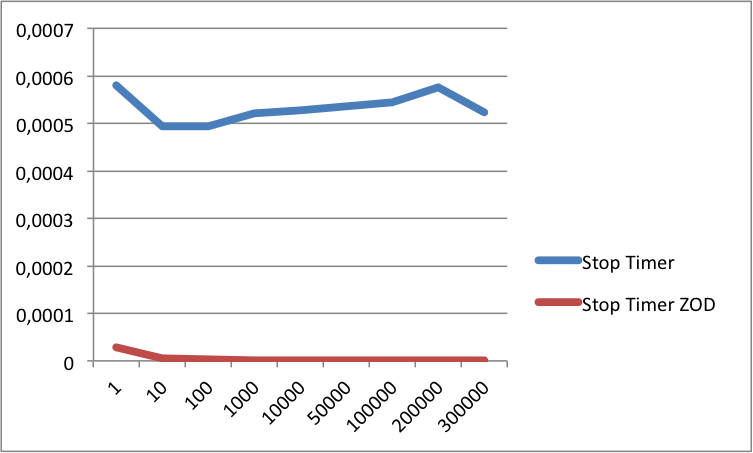
\includegraphics[scale=1.0]{Afbeeldingen/Evaluatie/StopTimer}
  \caption{Grafiek vergelijking tijden stoppen van een \texttt{Timer}.}
  \label{fig:GraphTimerStop}
\end{figure}

De figuur \ref{fig:GraphTimerStop} geeft de tijd dat het kost om een \texttt{Timer} te stoppen weer. Deze figuur geeft weer dat het stoppen van een \texttt{Timer} gemiddeld gezien evenveel tijd kost, ondanks dat het aantal simultane metingen verhoogd wordt. \\


\begin{figure}[h]
  \centering
  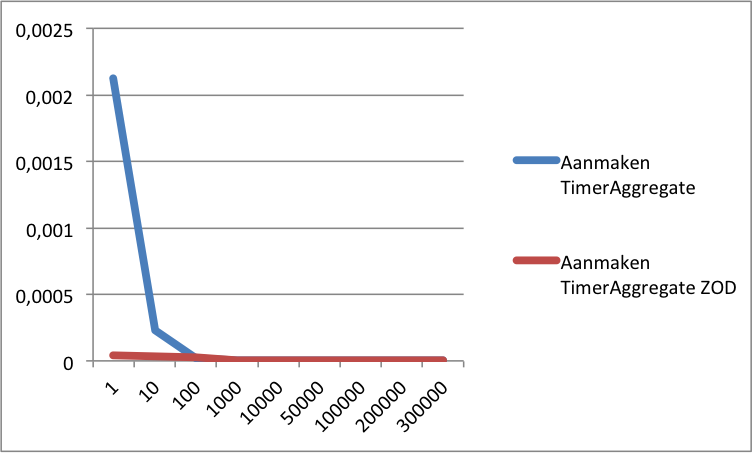
\includegraphics[scale=1.0]{Afbeeldingen/Evaluatie/AanmakenTimerAggregate}
  \caption{Grafiek vergelijking tijden aanmaken van een \texttt{TimerAggregate} object.}
  \label{fig:GraphTimerAggregate}
\end{figure}

De figuur \ref{fig:GraphTimerAggregate} geeft de tijd die het inneemt om een \texttt{TimerAggregate} object aan te maken weer. De negatieve invloed van het tijdelijk opslaan van de gegevens op de harde schijf wordt naarmate het aantal simultane metingen stijgt minimaal. \\

\begin{figure}[h]
  \centering
  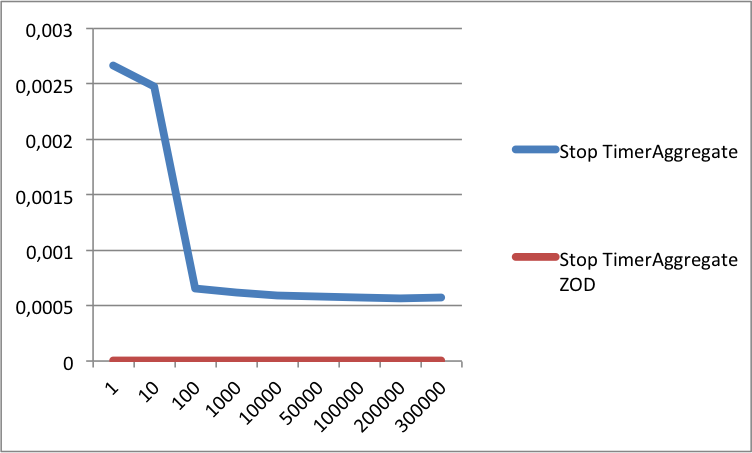
\includegraphics[scale=1.0]{Afbeeldingen/Evaluatie/StopTimerAggregate}
  \caption{Grafiek vergelijking tijden stoppen van een \texttt{TimerAggregate} object.}
  \label{fig:GraphTimerAggregateStop}
\end{figure}

De figuur \ref{fig:GraphTimerAggregateStop} geeft de tijd dat het kost om een \texttt{TimerAggregate} te stoppen weer. Deze figuur laat zien dat, net zoals het aanmaken van een \texttt{TimerAggregate}, de uitvoeringstijd eerst sterk daalt en daarna ongeveer hetzelfde blijft. Het verschil ligt erin dat het verschil in tijd tussen het opslaan van de gegevens op de harde schijf en het niet opslaan van de gegevens op de harde schijf bij het aanmaken van een \texttt{TimerAggregate} convergeert naar ongeveer dezelfde tijd, terwijl bij het stoppen van de \texttt{TimerAggregate} hier steeds een verschil tussen blijft bestaan. \\


\begin{figure}[h]
  \centering
  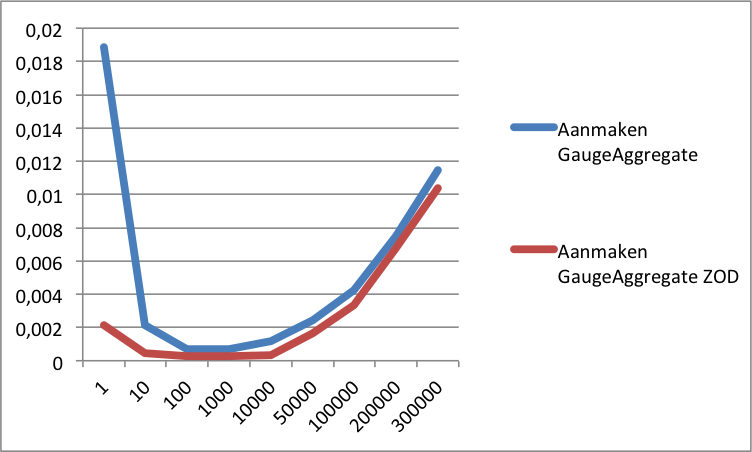
\includegraphics[scale=1.0]{Afbeeldingen/Evaluatie/AanmakenGaugeAggregate}
  \caption{Grafiek vergelijking tijden aanmaken van een \texttt{GaugeAggregate}.}
  \label{fig:GraphGaugeAggregate}
\end{figure}

De figuur \ref{fig:GraphGaugeAggregate} geeft de grafiek weer die het aanmaken van een \texttt{GaugeAggregate} weergeeft. In deze grafiek kan gezien worden dat verschil tussen het opslaan van de gegevens op de harde schijf en het niet opslaan van de gegevens op de harde schijf minimaal wordt indien een treshold bereikt wordt. \\


\subsection{Invloed op FPS}
De gemiddelde tijd om een methode uit te voeren zegt iets over de vertraging die de library extra invoert in de applicatie. Het zegt echter niets over de impact op de framerate van de applicatie. Om dit te kunnen testen werd er gekozen om de impact van de library op een game te testen. Zoals eerder vermeldt, is deze game een angry birds kloon. \\

Om deze test uit te voeren werd de volgende testopstelling gebruikt. Het gemiddeld aantal frames per second (FPS) wordt berekend uit 3000 gemeten waarden. Een FPS waarde wordt elke 0.2 seconde gemeten. Om de impact van de library op deze FPS te testen werd ervoor gekozen om elke seconde X aantal keer een library call uit te voeren en deze X gradueel te verhogen. Er werd gekozen om de worst case test uit te voeren gebaseerd op de test van de call duration. Het aanmaken van een \texttt{Counter} gecombineerd met het tijdelijk opslaan van de gegevens op de harde schijf heeft gemiddeld de grootste impact van de niet-geaggregeerde objecten. Om de invloed van de library op de FPS van de applicatie te onderzoeken zonder dat de metingen op de harde schijf opgeslagen worden, wordt het stoppen van een Timer gebruikt, omdat deze de grootste call duratie heeft van de niet-geaggregeerde objecten. \\

Een andere factor die invloed kan hebben op de impact die de library heeft op de applicatie, is het synchronisatieinterval. Dit interval vormt een indicatie van hoeveel tijd er zich tussen twee synchronisatiecycli bevindt. Door dit synchronisatieinterval systematisch te verlagen kan de invloed van de Tracklytics library op de FPS van de applicatie gemeten worden. \\


De resultaten van deze metingen zijn te vinden in de appendix \ref{Appendix}. Uit deze resultaten kan afgelezen worden dat de Tracklytics library een significante impact heeft op de applicatie indien het aantal simultane metingen groter wordt dan 20 en de gegevens tijdelijk op de harde schijf opgeslagen worden. Indien de gegevens niet op de harde schijf opgeslagen worden, dan heeft de Tracklytics library een significante impact op de applicatie als het aantal simultane metingen ongeveer 1000 betreft. \\


\section{Discussie Schaalbaarheid} \label{schaalbaarheid}
Een potenti\"ele bottleneck in de Tracklytics architectuur is de back end. Indien de load op de servers te groot wordt, zou ditimpact kunnen hebben op de applicatie. De Tracklytics library zou de netwerkinterface constant gebruiken om de metingen te synchroniseren naar de back end. De applicatie waarin de library wordt ingebouwd deelt deze netwerkinterface met de library. Als gevolg hiervan wordt de applicatie trager, omdat de netwerkinterface constant gebruikt wordt door de library. Dit scenario moet voorkomen worden om de bruikbaarheid van de Tracklytics library optimaal te houden.\\

Een oplossing voor dit probleem is de back end uit te schalen over meerdere servers en servers bij te voegen indien de load op de servers te groot wordt. Om de back end schaalbaar te maken moet zowel de PHP code die op de servers draait schaalbaar zijn, alsook de database die in de back end draait. \\

De PHP code verwerkt de metingen komende van de Tracklytics library en zet deze resultaten in de database. Voor deze code is het voldoende dat deze een connectie tot een database hebben en dit maakt de PHP code dus zeer schaalbaar.\\

De database gebruikt in de Tracklytics library is een MySQL database. Dit is een implementatie van een Relational database management system (RDBMS). Een alternatief hiervoor zou zijn om een NoSQL database te gebruiken. Dit soort database werd ontwikkeld om schaalbaar te zijn. Het nadeel hiervan is dat de ACID properties niet gegarandeerd kunnen worden, wat ervoor zorgt dat data inconsistent kan worden. Er bestaat ook nog geen standaard taal (zoals SQL voor RDBMS), zodat de overgang van een RDBMS (of van een andere NoSQL) naar een NoSQL database een probleem kan vormen. \\


\section{Developer effort Evaluatie}\label{Section:Effort}
Met DevOps willen developers en managers het ontwikkelingsproces van software versnellen. Het is ongewenst dat het veel effort om de library in de applicatie in te bouwen, omdat dit enerzijds meer tijd inneemt om de code te schrijven en anderzijds de code minder overzichtelijk maakt voor de developers. \\

Om deze eigenschappen na te gaan werd ervoor gekozen om volgende zaken na te gaan: hoeveel tijd neemt het in om de library in te bouwen, het aantal lijnen code nodig om deze in de applicatie in te bouwen, wat er gemonitord wordt en hoeveel metingen er maximaal simultaan voorkomen. Met ''hoeveel tijd neemt het in om de library in te bouwen''  wordt de gehele flow bedoeld: het registreren van de applicatie in de back end, het installeren van de library via CocoaPods en het implementeren van de code in de applicatie. \\

Om deze zaken na te gaan, zijn er twee applicaties gebruikt, namelijk de stopwatch applicatie die eerder vermeldt werd en een applicatie ontwikkeld in mijn stage. De volgende tabel geeft de eigenschappen van deze applicaties weer \ref{table:apps}.

\begin{table}[h]
\centering
\caption{Eigenschappen van twee gebruikte test applicaties.}
\label{table:apps}
\begin{tabular}{lll}
                     & \#lijnen code & ontwikkelingstijd \\
stopwatch applicatie & 250           & 10 minuten        \\
tweede applicatie    & 10000         & 4 maanden        
\end{tabular}
\end{table}

\subsection{Resultaten}
In deze sectie worden de resultaten besproken van de evaluatie van de developer effort.\\
In de stopwatch applicatie worden volgende zaken gemonitord: alle buttons, tijd wanneer op stop gedrukt, aantal rondes alvorens reset, tijd om data van een server te halen. In de andere applicatie worden volgende zaken gemonitord: alle buttons waarop geklikt wordt, alle screen visits, \#zoekresultaten, duratie van complexe code, duratie content van het netwerk halen.\\

\begin{table}[h]
\centering
\caption{Resultaten developer effort.}
\label{table:effort}
\begin{tabular}{llllll}
                     & \begin{tabular}[c]{@{}l@{}}duratie \\ implementatie\end{tabular} & \#meetobjecten & \begin{tabular}[c]{@{}l@{}}Gemiddeld aantal\\ lijnen per meetobject\end{tabular} & \begin{tabular}[c]{@{}l@{}}totaal aantal\\ lijnen code\end{tabular} & \begin{tabular}[c]{@{}l@{}}Maximaal aantal\\ simultane metingen\end{tabular} \\
stopwatch applicatie & \textless10 minuten                                              & 9              & 1.0                                                                              & 9                                                                   & 2                                                                            \\
tweede applicatie    & + 90 minuten                                                     & 68             & 1.4                                                                              & 100                                                                 & 10                                                                          
\end{tabular}
\end{table}

Uit deze resultaten kan afgeleid worden dat de developer effort om de Tracklytics library in de applicatie in te bouwen minimaal is. Voor de stopwatch applicatie neemt het inbouwen van de library maar \underline{+} 1\% van de tijd in beslag. Voor de andere applicatie is er geen percentage berekenbaar, maar anderhalf uur op vier maanden is zeker laag genoeg om geen significante impact te hebben op het developen van een applicatie. Het aantal lijnen code dat extra moet geschreven worden is 3.6\% in het geval van een kleine applicatie (de sportstimer) en ongeveer 1\% bij het ontwikkelen van een grotere applicatie (de andere applicatie). \\


Het is nuttig om dit soort informatie te meten, omdat met behulp van dit soort metingen kan ondervonden worden hoe de gebruiker de applicatie gebruikt. Er kan zo een overzicht gevormd worden welke knoppen hoe vaak gebruikt worden en welke schermen dat de gebruiker het vaakst bezoekt. Anderzijds vormt het monitoren van de duratie van complexe code en van het ophalen van informatie van het netwerk een manier om bottlenecks te kunnen ontdekken in de applicatie. 

\section{Conclusie en bespreking resultaten}\label{Section:Conclusie}
Zoals eerder besproken in deze thesis geeft de Tracklytics library de keuze aan de developer om de data op het toestel of in de back end te aggregeren. We hebben de metingen vergeleken van de geaggregeerde en de niet-geaggregeerde objecten. Indien we deze grafieken bekijken, dan kunnen we deze opdelen in twee verschillende secties, namelijk langs de ene kant de grafieken die te maken hebben met de \texttt{Gauge} en langs de andere kant de grafieken die te maken hebben met de \texttt{Meter} en de \texttt{Timer}. \\


\begin{figure}[h]
  \centering
  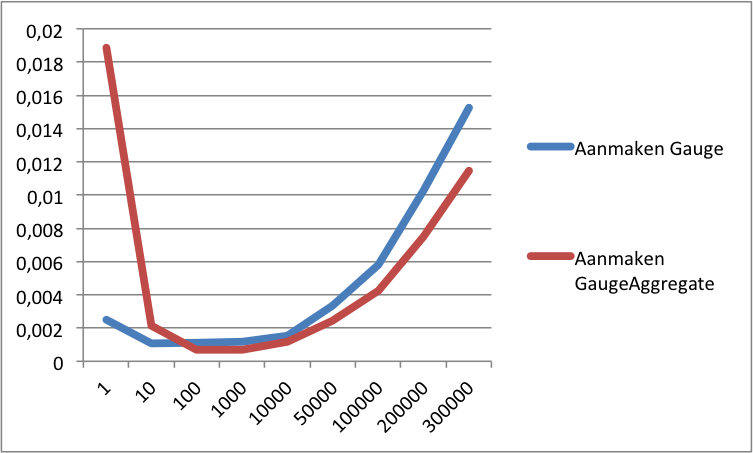
\includegraphics[scale=1.0]{Afbeeldingen/Evaluatie/GaugeVSAggregate}
  \caption{Grafiek vergelijking tussen het aanmaken van een \texttt{Gauge} en een \texttt{GaugeAggregate} object.}
  \label{fig:GaugeVSAggregate}
\end{figure}

\begin{figure}[h]
  \centering
  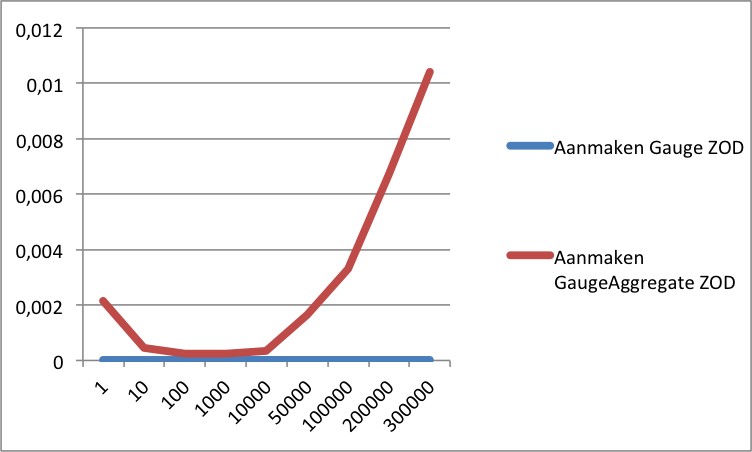
\includegraphics[scale=1.0]{Afbeeldingen/Evaluatie/GaugeVSAggregateZOD}
  \caption{Grafiek vergelijking tussen het aanmaken van een \texttt{Gauge} en een \texttt{GaugeAggregate} object zonder opslaan op de harde schijf.}
  \label{fig:GaugeVSAggregateZOD}
\end{figure}



Bekijken we de grafieken in verband met de \texttt{Gauge}: \ref{fig:GaugeVSAggregate}, \ref{fig:GaugeVSAggregate}, dan kunnen we daar het volgende uit afleiden: de tijd om een \texttt{GaugeAggregate} aan te maken daalt eerst tot en met er ongeveer 100 metingen simultaan gebeuren en stijgt dan later vanaf ongeveer 10000 simultane metingen opnieuw. De reden hiervoor is dat de Tracklytics library een lijst van alle waarden bij houdt in de \texttt{GaugeAggregate} klasse om de exacte mediaan te kunnen berekenen. \\

\begin{figure}[h]
  \centering
  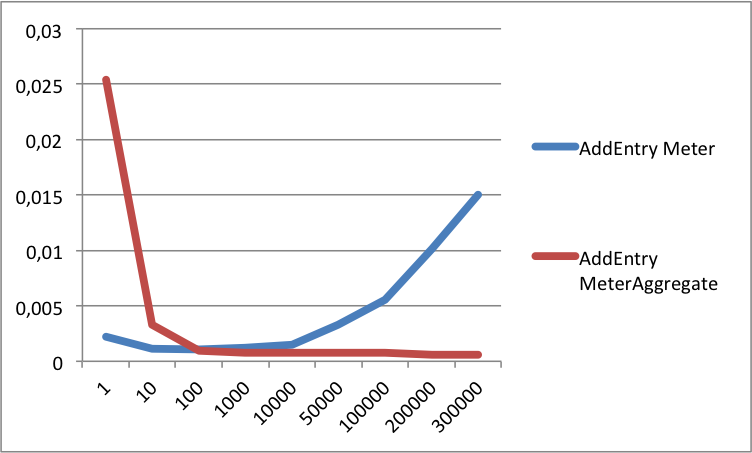
\includegraphics[scale=1.0]{Afbeeldingen/Evaluatie/MeterVSAggregate}
  \caption{Grafiek vergelijking tussen het aanmaken van een \texttt{Meter} en een \texttt{MeterAggregate} object.}
  \label{fig:MeterVSAggregate}
\end{figure}

\begin{figure}[h]
  \centering
  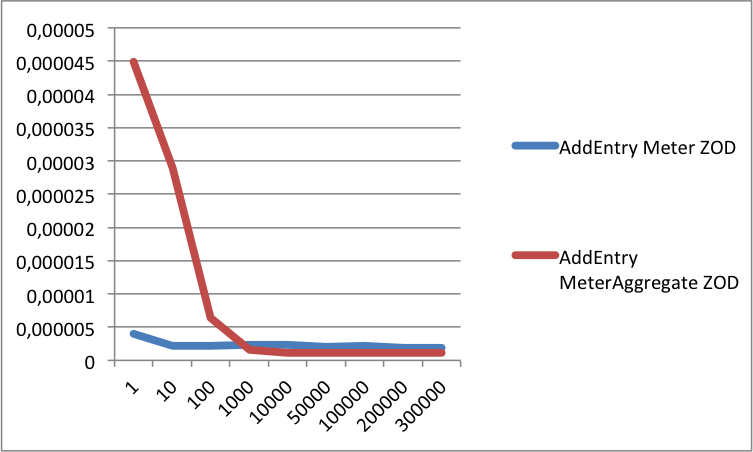
\includegraphics[scale=1.0]{Afbeeldingen/Evaluatie/MeterVSAggregateZOD}
  \caption{Grafiek vergelijking tussen het aanmaken van een \texttt{Meter} en een \texttt{MeterAggregate} object zonder opslaan op de harde schijf.}
  \label{fig:MeterVSAggregateZOD}
\end{figure}

De grafieken \ref{fig:MeterVSAggregate} en \ref{fig:MeterVSAggregateZOD} geven de vergelijking tussen het aanroepen van de \texttt{addEntry} methode op een \texttt{Meter} en het aanroepen van de \texttt{addEntry} methode op een \texttt{MeterAggregate} weer. Hieruit kan afgeleid worden dat indien het aantal simultane metingen lager dan 100 blijft, het effici\"enter is om de niet-geaggregeerde objecten te gebruiken. \\

\begin{figure}[h]
  \centering
  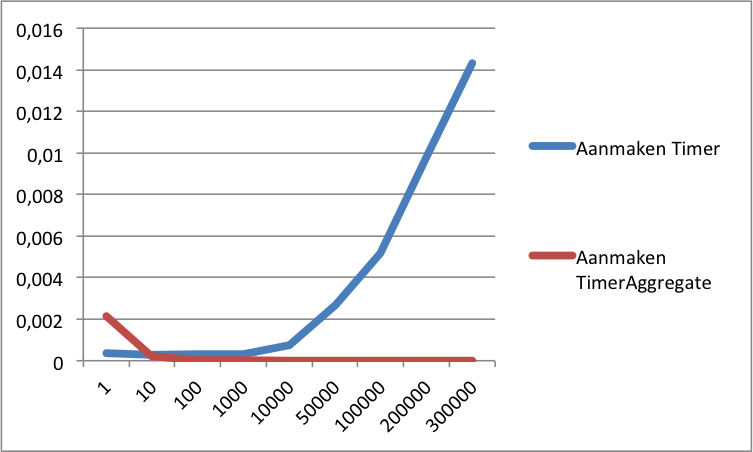
\includegraphics[scale=1.0]{Afbeeldingen/Evaluatie/TimerVSAggregate}
  \caption{Grafiek vergelijking tussen het aanmaken van een \texttt{Timer} en een \texttt{TimerAggregate} object.}
  \label{fig:TimerVSAggregate}
\end{figure}

\begin{figure}[h]
  \centering
  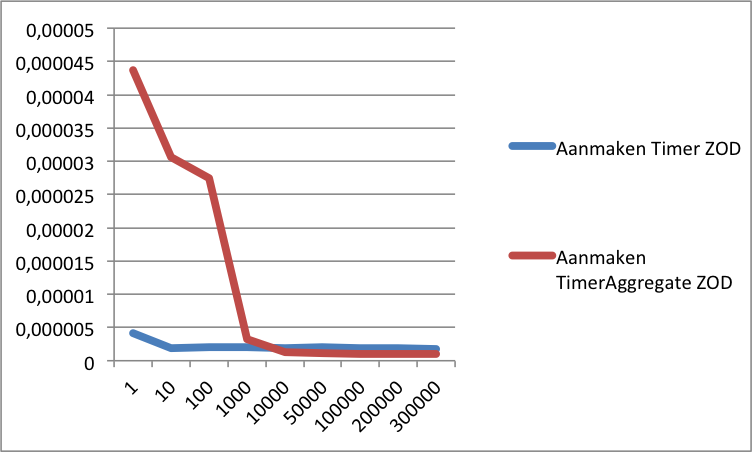
\includegraphics[scale=1.0]{Afbeeldingen/Evaluatie/TimerVSAggregateZOD}
  \caption{Grafiek vergelijking tussen het aanmaken van een \texttt{Timer} en een \texttt{TimerAggregate} object zonder opslaan op de harde schijf.}
  \label{fig:TimerVSAggregateZOD}
\end{figure}

De grafieken \ref{fig:TimerVSAggregate} en \ref{fig:TimerVSAggregateZOD} geven de vergelijking tussen het aanmaken van een \texttt{Timer} object en het aanmaken van een \texttt{TimerAggregate} object weer. Uit deze grafieken kan afgeleid worden dat tot ongeveer 1000 simultane metingen het effici\"enter of ongeveer effici\"ent is om het niet-geaggregeerde object te gebruiken. \\

\begin{figure}[h]
  \centering
  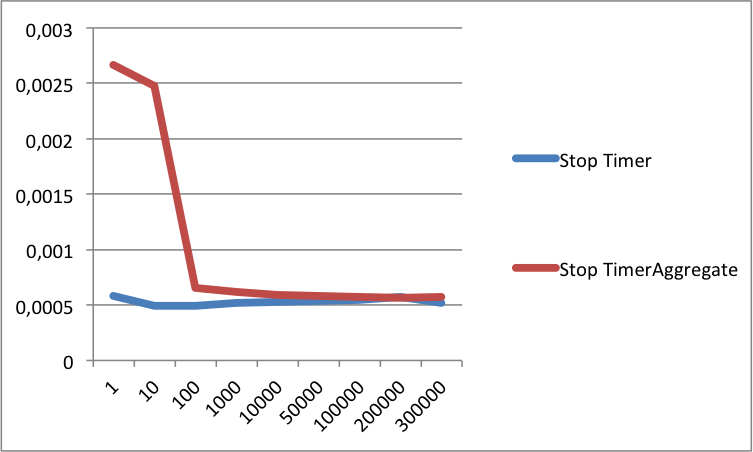
\includegraphics[scale=1.0]{Afbeeldingen/Evaluatie/StopVSTimerAggregate}
  \caption{Grafiek vergelijking tussen het aanroepen van de stop methode op een \texttt{Timer} en het aanroepen van de stop methode op een \texttt{TimerAggregate} object.}
  \label{fig:StopVSTimerAggregate}
\end{figure}

\begin{figure}[h]
  \centering
  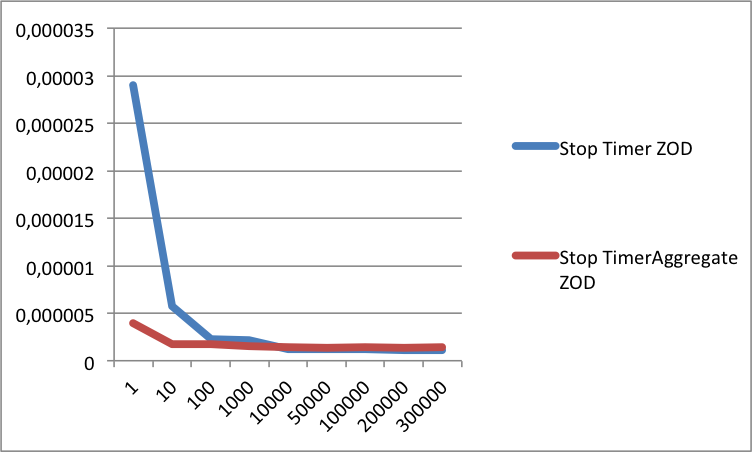
\includegraphics[scale=1.0]{Afbeeldingen/Evaluatie/StopVSTimerAggregateZOD}
  \caption{Grafiek vergelijking tussen het aanroepen van de stop methode op een \texttt{Timer} en het aanroepen van de stop methode op een \texttt{TimerAggregate} object zonder opslaan op de harde schijf..}
  \label{fig:StopVSTimerAggregateZOD}
\end{figure}
De grafieken \ref{fig:StopVSTimerAggregate} en \ref{fig:StopVSTimerAggregateZOD} geven de vergelijking tussen het aanroepen van de \texttt{stop} methode op een \texttt{Timer} en het aanroepen van de \texttt{stop} methode op een \texttt{TimerAggregate} weer. Deze grafieken geven weer dat, indien de data tijdelijk wordt opgeslagen op de harde schijf, het niet-aggregeren van de data effici\"enter is dan het aggregeren van de data. Indien de data niet op de harde schijf opgeslagen wordt, is het tot en met 100 simultane metingen effici\"enter om de data te aggregeren op het toestel. Indien er een groter aantal metingen simultaan gebeurt is het aggregeren van de data ongeveer even effici\"ent als het niet aggregeren van de data. \\

Uit deze observaties kan afgeleid worden dat, indien het aantal simultane metingen onder de 100 blijft, het meestal effici\"enter is om de data niet te aggregeren. Enkel het stoppen van een \texttt{TimerAggregate} is in dit geval sneller. \\


Bekijken we de resultaten van hoeveel effort een developer in een applicatie moet stoppen (\ref{Section:Effort}), concluderen we dat bij een grote applicatie er ongeveer 10 metingen tegelijk kunnen gebeuren. Indien we dit resultaat combineren met de resultaten van de grafieken en cijfers van de metingen van de geaggregeerde objecten, zien we dat, met uitzondering tot het stoppen van een Timer, het steeds het geval is dat het niet aggregeren van de metingen op het toestel sneller of ongeveer even snel is als het aggregeren van de metingen op het toestel tot en met 100 simultane metingen. Uit deze observatie kunnen we afleiden dat het aggregeren van de metingen op het toestel van de gebruiker een grotere performance impact heeft dan het aggregeren van de metingen in de back end. \\

Naast het evalueren van de call duratie van de Tracklytics library hebben we de impact op de FPS van de Tracklytics library ge\"evalueerd. Indien we deze resultaten bekijken, bekomen we dat tot en met 20 simultane metingen, de impact op de applicatie van de library minimaal is indien de gegevens op de harde schijf opgeslagen worden. Het aantal FPS daalt pas significant indien het aantal simultane metingen richting 50 gaat. Indien de gegevens niet op de harde schijf opgeslagen worden, heeft de library een minimale invloed op de applicatie. Deze observatie zorgt ervoor dat, in het geval dat FPS de limiterende factor is, de library in elke applicatie ingebouwd kan worden indien het maximum aantal simultane metingen in de buurt van 20 ligt, indien de developer wil dat alle gegevens tijdelijk op de harde schijf van de applicatie opgeslagen worden. \\ 

Een gebruiker merkt een vertraging pas indien de vertraging groter wordt dan 0.1 seconde \cite{nielsen1994usability}. De Tracklytics library zou dit getal niet mogen overstijgen om de impact op de performance aanvaardbaar te houden. In de resultaten van de call duratie zien we dat bij elk meetobject 100 simultane uitvoeringen gedaan moeten worden om de 0.1 seconde vertraging te overstijgen indien de metingen op de harde schijf van de telefoon opgeslagen worden. \\


Uit deze observaties kunnen we concluderen dat de library bruikbaar is op het vlak van performance bij het ontwikkelen van een applicatie, zelfs indien de data op de harde schijf opgeslagen wordt. De developers moeten er rekening mee houden dat er maximaal rond de \textbf{20 simultane metingen} in de applicatie mogen gebeuren om de vertraging van de applicatie binnen de perken te houden indien de data tijdelijk op de harde schijf opgeslagen wordt. Indien de metingen niet op de harde schijf opgeslagen worden alvorens te synchroniseren naar de back end, dan staat er geen \'echte limiet op het aantal simultane metingen. Meer dan 1000 simultane metingen zijn mogelijk in deze situatie alvorens de library een significante impact heeft op de prestaties van de applicatie. \\

De effort van de developer moet met een korrel zout genomen worden, omdat de ontwikkelaar van de library deze testen zelf heeft uitgevoerd. Het is waarschijnlijk dat developers een langere tijd nodig hebben om de Tracklytics library in te bouwen in een applicatie. \\












%%% Local Variables: 
%%% mode: latex
%%% TeX-master: "masterproef"
%%% End: 
